
%%\documentclass[12pt,preprint]{aastex}

%% manuscript produces a one-column, double-spaced document:

%% \documentclass[10pt,manuscript]{aastex}

%% preprint2 produces a double-column, single-spaced document:
\documentclass[preprint2,iop,numberedappendix,twocolappendix,appendixfloats]{emulateapj}
%% \documentclass[preprint2,iop]{aastex}

%% \documentclass[preprint2,longabstract]{aastex}

%% \usepackage{ccaption}
%% \captionstyle{\raggedright}
\usepackage[caption=false]{subfig}
\usepackage{amsmath}
\usepackage{footnote}
\bibpunct{(}{)}{;}{a}{}{,} 
\captionsetup{belowskip=12pt,aboveskip=4pt}
\setlength{\textfloatsep}{10pt plus 1.0pt minus 2.0pt}
\newcommand{\dif}{\mathrm{d}}
%% \renewcommand*{\thefootnote}{\fnsymbol{footnote}}

\def\nar{{New~A~Rev.}}          % New Astronomy Review
\def\pasa{{PASA}}               % Publications of the Astron. Soc. of Australia

%% \bibliographystyle{mn2e}
%% \bibliographystyle{apj}

\shorttitle{Effects of Beam Chromaticity in EoR Power Spectra Measurements}
\shortauthors{Thyagarajan et~al.}

\def\ASU{\altaffilmark{1}}
\def\ASUtxt{\altaffiltext{1}{Arizona State University, School of Earth and Space Exploration, Tempe, AZ 85287, USA}}

\def\myemail{\altaffilmark{*}}
\def\myemailtxt{\altaffiltext{*}{e-mail: t\_nithyanandan@asu.edu}}

\def\UW{\altaffilmark{2}}
\def\UWtxt{\altaffiltext{2}{University of Washington, Department of Physics, Seattle, WA 98195, USA}}

\def\SKASA{\altaffilmark{3}}
\def\SKASAtxt{\altaffiltext{3}{Square Kilometre Array South Africa (SKA SA), Park Road, Pinelands 7405, South Africa}}

\def\RU{\altaffilmark{4}}
\def\RUtxt{\altaffiltext{4}{Department of Physics and Electronics, Rhodes University, Grahamstown 6140, South Africa}}

\def\CfA{\altaffilmark{5}}
\def\CfAtxt{\altaffiltext{5}{Harvard-Smithsonian Center for Astrophysics, Cambridge, MA 02138, USA}}

\def\ANU{\altaffilmark{6}}
\def\ANUtxt{\altaffiltext{6}{Australian National University, Research School of Astronomy and Astrophysics, Canberra, ACT 2611, Australia}}

\def\CAASTRO{\altaffilmark{7}}
\def\CAASTROtxt{\altaffiltext{7}{ARC Centre of Excellence for All-sky Astrophysics (CAASTRO)}}

\def\Haystack{\altaffilmark{8}}
\def\Haystacktxt{\altaffiltext{8}{MIT Haystack Observatory, Westford, MA 01886, USA}}

\def\MIT{\altaffilmark{9}}
\def\MITtxt{\altaffiltext{9}{MIT Kavli Institute for Astrophysics and Space Research, Cambridge, MA 02139, USA}}

\def\Curtin{\altaffilmark{10}}
\def\Curtintxt{\altaffiltext{10}{International Centre for Radio Astronomy Research, Curtin University, Perth, WA 6845, Australia}}

\def\Victoria{\altaffilmark{11}}
\def\Victoriatxt{\altaffiltext{11}{Victoria University of Wellington, School of Chemical \& Physical Sciences, Wellington 6140, New Zealand}}

\def\UWisc{\altaffilmark{12}}
\def\UWisctxt{\altaffiltext{12}{University of Wisconsin--Milwaukee, Department of Physics, Milwaukee, WI 53201, USA}}

\def\UMichigan{\altaffilmark{13}}
\def\UMichigantxt{\altaffiltext{13}{University of Michigan, Department of Atmospheric, Oceanic and Space Sciences, Ann Arbor, MI 48109, USA}}

\def\UMelbourne{\altaffilmark{14}}
\def\UMelbournetxt{\altaffiltext{14}{The University of Melbourne, School of Physics, Parkville, VIC 3010, Australia}}

\def\USydney{\altaffilmark{15}}
\def\USydneytxt{\altaffiltext{15}{The University of Sydney, Sydney Institute for Astronomy, School of Physics, NSW 2006, Australia}}

\def\CASS{\altaffilmark{16}}
\def\CASStxt{\altaffiltext{16}{CSIRO Astronomy and Space Science (CASS), PO Box 76, Epping, NSW 1710, Australia}}

\def\Tata{\altaffilmark{17}}
\def\Tatatxt{\altaffiltext{17}{National Centre for Radio Astrophysics, Tata Institute for Fundamental Research, Pune 411007, India}}

\def\RRI{\altaffilmark{18}}
\def\RRItxt{\altaffiltext{18}{Raman Research Institute, Bangalore 560080, India}}

\def\NRAO{\altaffilmark{19}}
\def\NRAOtxt{\altaffiltext{19}{National Radio Astronomy Observatory, Charlottesville and Greenbank, USA}}

\def\UWA{\altaffilmark{20}}
\def\UWAtxt{\altaffiltext{20}{International Centre for Radio Astronomy Research, University of Western Australia, Crawley, WA 6009, Australia}}

%% \definenote[thanks][conversion=set 2]

\begin{document}

\title{Effect of Beam Chromaticity on Foregrounds in Wide-Field Measurements of Redshifted 21~cm Power Spectra}

%% Use \author, \affil, and the \and command to format
%% author and affiliation information.
%% Note that \email has replaced the old \authoremail command
%% from AASTeX v4.0. You can use \email to mark an email address
%% anywhere in the paper, not just in the front matter.
%% As in the title, use \\ to force line breaks.

%% Author list
\author{
%% Lead Authors
Nithyanandan~Thyagarajan\ASU\myemail,
TBD
% Daniel~C.~Jacobs\ASU,
% Judd~D.~Bowman\ASU,
% N.~Barry\UW,
% A.~P.~Beardsley\UW,
% G.~Bernardi\SKASA$^,$\RU$^,$\CfA,
% F.~Briggs\ANU$^,$\CAASTRO,
% R.~J.~Cappallo\Haystack, 
% P.~Carroll\UW,
% B.~E.~Corey\Haystack, 
% % A.~A.~Deshpande\RRI, 
% A.~de~Oliveira-Costa\MIT,
% Joshua~S.~Dillon\MIT,
% D.~Emrich\Curtin,
% % B.~M.~Gaensler\USydney$^,$\CAASTRO, 
% A.~Ewall-Wice\MIT,
% L.~Feng\MIT,
% R.~Goeke\MIT,
% L.~J.~Greenhill\CfA,
% B.~J.~Hazelton\UW, 
% J.~N.~Hewitt\MIT,
% N.~Hurley-Walker\Curtin,
% M.~Johnston-Hollitt\Victoria,
% D.~L.~Kaplan\UWisc, 
% J.~C.~Kasper\UMichigan$^,$\CfA, 
% Han-Seek Kim\UMelbourne$^,$\CAASTRO,
% P.~Kittiwisit\ASU,
% E.~Kratzenberg\Haystack, 
% E.~Lenc\USydney$^,$\CAASTRO,
% J.~Line\UMelbourne$^,$\CAASTRO,
% A.~Loeb\CfA,
% C.~J.~Lonsdale\Haystack, 
% M.~J.~Lynch\Curtin, 
% B.~McKinley\UMelbourne$^,$\CAASTRO,
% S.~R.~McWhirter\Haystack,
% D.~A.~Mitchell\CASS$^,$\CAASTRO, 
% M.~F.~Morales\UW, 
% E.~Morgan\MIT, 
% A.~R.~Neben\MIT,
% D.~Oberoi\Tata, 
% A.~R.~Offringa\ANU$^,$\CAASTRO, 
% S.~M.~Ord\Curtin$^,$\CAASTRO,
% Sourabh Paul\RRI,
% B.~Pindor\UMelbourne$^,$\CAASTRO,
% J.~C.~Pober\UW,
% T.~Prabu\RRI, 
% P.~Procopio\UMelbourne$^,$\CAASTRO,
% J.~Riding\UMelbourne$^,$\CAASTRO,
% A.~E.~E.~Rogers\Haystack, 
% A.~Roshi\NRAO, 
% N.~Udaya~Shankar\RRI, 
% Shiv~K.~Sethi\RRI,
% K.~S.~Srivani\RRI, 
% R.~Subrahmanyan\RRI$^,$\CAASTRO, 
% I.~S.~Sullivan\UW,
% M.~Tegmark\MIT,
% S.~J.~Tingay\Curtin$^,$\CAASTRO, 
% C.~M.~Trott\Curtin$^,$\CAASTRO,
% M.~Waterson\Curtin$^,$\ANU,
% R.~B.~Wayth\Curtin$^,$\CAASTRO, 
% R.~L.~Webster\UMelbourne$^,$\CAASTRO, 
% A.~R.~Whitney\Haystack, 
% A.~Williams\Curtin, 
% C.~L.~Williams\MIT,
% C.~Wu\UWA,
% J.~S.~B.~Wyithe\UMelbourne$^,$\CAASTRO
}

%Institutional footnotes (typeset, then rearrange here to be in order)
\ASUtxt
% \UWtxt
% \SKASAtxt
% \RUtxt
% \CfAtxt
% \ANUtxt
% \CAASTROtxt
% \Haystacktxt
% \MITtxt
% \Curtintxt
% \Victoriatxt
% \UWisctxt
% \UMichigantxt
% \UMelbournetxt
% \USydneytxt
% \CASStxt
% \Tatatxt
% \RRItxt
% \NRAOtxt
% \UWAtxt
\myemailtxt

%% \clearpage

\begin{abstract}

\end{abstract}
 
\keywords{cosmology: observations --- dark ages, reionization, first stars --- large-scale structure of universe --- methods: statistical --- radio continuum: galaxies --- techniques: interferometric}

\section{Introduction}\label{intro}

The period in the history of the Universe characterized by the transition of neutral hydrogen in the intergalactic medium (IGM) to a fully ionized state due to the formation of radiating objects such as the first stars and galaxies is referred to as the Epoch of Reionization (EoR). This is an important period of nonlinear growth of matter density perturbations and astrophysical evolution leading to the large scale structure observed currently in the Universe. And yet, this period in the Universe's history has remained poorly probed to date with observations. 

The redshifted neutral hydrogen from the IGM in this epoch has been identified to be one of the most promising and direct probes of the EoR \citep{sun72,sco90,mad97,toz00,ili02}. Numerous experiments using low frequency radio telescopes targeting the redshifted 21~cm line from the spin-flip transition of H{\sc i} have become operational such as the Murchison Widefield Array \citep[MWA;][]{lon09,bow13,tin13}, the Precision Array for Probing the Epoch of Reionization \citep[PAPER;][]{par10}, the Low Frequency Array \citep[LOFAR;][]{van13} and the Giant Metrewave Radio Telescope EoR experiment \citep[GMRT;][]{pac13}. These instruments have sufficient sensitivity for a statistical detection of the EoR signal via estimating the spatial power spectrum of the redshifted H{\sc i} temperature fluctuations \citep{bea13,thy13}. These instruments are intended to be precursors and pathfinders to the next generation of low frequency radio observatories such as the Hydrogen Epoch of Reionization Array\footnote{\url{http://reionization.org/}} (HERA; DeBoer~et~al.~2015) and the Square Kilometre Array\footnote{\url{https://www.skatelescope.org/}} (SKA). These next-generation instruments will advance the capability from a mere statistical detection of the signal to a direct three-dimensional tomographic imaging of the H{\sc i} during the EoR. 

The most significant challenge to low frequency EoR observations arises from the extremely bright Galactic and extragalactic foreground synchrotron emission which are $\sim 10^4$ times stronger than the desired EoR signal \citep{dim02,ali08,ber09,ber10,gho12}. All the current and future instruments rely on the inherent differences in spatial isotropy and spectral smoothness between the EoR signal and the foregrounds to extract the EoR power spectrum \citep[see, e.g.,][]{fur04,mor04,zal04,san05,fur06,mcq06,mor06,wan06,gle08}. 

When expressed in the coordinate system of power spectrum measurements described by the three-dimensional wavenumber ($k$), the foreground emission is restricted to a wedge-shaped region commonly referred to as the {\it foreground wedge} \citep{bow09,liu09,liu14a,liu14b,dat10,liu11,gho12,mor12,par12b,tro12,ved12,dil13,pob13,thy13,dil14} whereas the EoR signal has spherical symmetry due to its isotropy which appears elongated along line of sight $k$ modes due to peculiar velocity effects when dominated by matter density perturbations during early stages of reionization. 

The extreme dynamic range required to subtract foregrounds precisely demands high precision modeling of foregrounds as observed by modern wide-field instruments \citep{thy15a,thy15b}. Their studies of effects of wide-field measurements of EoR power spectra have demonstrated the {\it pitchfork} effect wherein foreshortening of baselines causes a prominent enhancement of foreground power near the horizon limits of the {\it foreground wedge} as well in the contamination beyond. In this paper, we explore yet another phenomenon that inherently extends foreground power beyond the {\it wedge}, namely, that arising from the chromaticity of the antenna power pattern. % We specifically use the current design of 14~m dish of HERA as an example in our study.

This paper is organized as follows. \S\ref{sec:HERA} introduces the HERA instrument. A brief summary of the delay spectrum technique used extensively in this analysis and the recently confirmed {\it pitchfork} effect are presented in \S\ref{sec:delay-spectrum}. \S\ref{sec:sim} describes foreground simulations including antenna beam pattern and all-sky foreground models. \S\ref{sec:beam-chromaticity} investigates the effects of chromaticity of antenna beam on the resulting delay power spectrum and the cosmologically motivated constraints it places on dish reflectometry. Our findings are summarized in \S\ref{sec:summary}.

\section{The Hydrogen Epoch of Reionization Array}\label{sec:HERA}

DeBoer~et~al.(2016)

\section{Delay Spectrum}\label{sec:delay-spectrum}

\citep{par12b}

\subsection{The Wide-Field ``Pitchfork'' Effect}\label{sec:wide-field}

\citep{thy15a,thy15b}

\section{Simulations}\label{sec:sim}

We simulate wide-field visibilities for 19-element HERA from all-sky antenna power pattern and foreground models using the PRISim\footnote{The Precision Radio Interferometry Simulator (PRISim) is publicly available at \href{https://github.com/nithyanandan/PRISim}{https://github.com/nithyanandan/PRISim}} software package. The simulations cover 24~hr of observation in {\it drift} mode consisting of 80 accumulations spanning 1080~s each. The total bandwidth is 100~MHz centered on 150~MHz consisting of 128 channels with 781.125~kHz frequency resolution each. Models of the antenna power pattern and foregrounds are described below.

\subsection{Antenna Power Pattern}

\citep{neb15}

\subsection{Foreground Model}\label{sec:foreground}

Our all-sky foreground model is the same as the one in \citet{thy15a}. It consists of diffuse emission \citep{deo08} and point sources. The latter is obtained from a combination of the NRAO VLA Sky Survey \citep[NVSS;][]{con98} at 1.4~GHz and the Sydney University Molonglo Sky Survey \citep[SUMSS;][]{boc99,mau03} at 843~MHz with a mean spectral index of -0.83. The diffuse sky model has an angular resolution of 13\farcm 74.

\section{Chromaticity of Power Pattern}\label{sec:beam-chromaticity}

The equation for delay spectrum describes the mapping between sky location of a foreground object and delay. The chromatic nature (variation with frequency) of the antenna power pattern results in a convolution of the geometrical mapping with the delay response of spectral chromaticity of the power pattern. This can result in a significant spillover of foreground power beyond the horizon delay limits especially in the case of foregrounds near the horizon. 

Fig.~\ref{fig:off-axis-beam-chromaticity} demonstrates the beyond-the-horizon spillover even from a flat-spectrum point source at different off-axis angles. The three panels correspond to delay spectra from different positions of the point source -- 0\arcdeg (left), 45\arcdeg (middle) and 89\arcdeg (right) -- from the zenith. The phase centers are located at the source positions and hence the delay spectra are centered on $\tau = 0$~ns. The response of the simulated dish power pattern (dashed line) is comapred with that from an {\it Airy} pattern resulting from a nominal uniformly illuminated circular disk (solid line). The gray vertical lines correspond to the horizon limits at $\pm 48.7$~ns for a 14.6~m antenna spacing. In all these cases, a {\it Blackman-Harris} window function has been applied along the spectral axis. 

\begin{figure*}[htb]
\centering
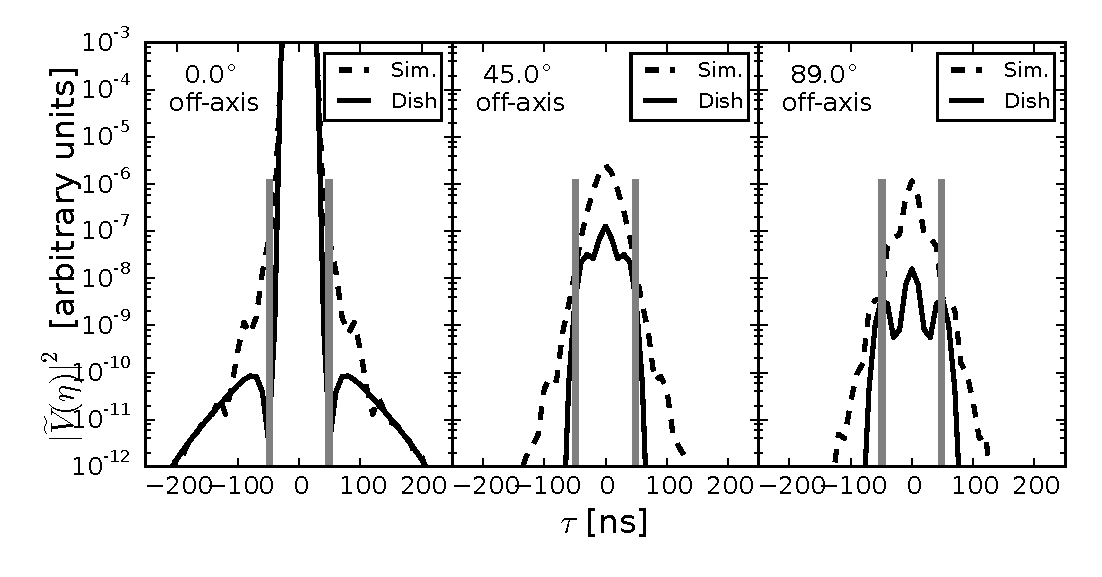
\includegraphics[width=\linewidth]{off-axis_point_source_beam_chromaticity.eps}
\caption{Chromaticity of antenna power pattern at directions off-axis. }
\label{fig:off-axis-beam-chromaticity}
\end{figure*}

At 0\arcdeg off-axis, the {\it Airy} pattern has no spectral variation except that introduced by the {\it Blackman-Harris} window function and thus reproduces its Fourier response centered at $\tau = 0$~ns whereas the simulated power pattern is found to exhibit some spectral variation giving rise to the wings on either side of $\tau = 0$~ns. As off-axis angle increases to 45\arcdeg, both the power patterns clearly exhibit chromaticity. The simulated pattern not only has a higher magnitude inside the horizon limits (by a factor $\sim 10$) but also exhibits higher chromaticity (by many orders of magnitude) in modes beyond the horizon relative to that of an {\it Airy} pattern. In contrast, at 89\arcdeg off-axis, not only does the simulated pattern have higher chromaticity in high delay modes but is also two orders of magnitude higher in amplitude inside the horizon limits relative to the nominal {\it Airy} pattern.

It is important to note that in a generic scenario where visibilities are not phased to a specific foreground location, the chromaticity of the power pattern will imprint itself on location of the foreground objects in delay space and will give rise to significant spillover especially from foregrounds near the horizon. 

We investigate the effects of spectral chromaticity of the power pattern in more detail below.

\subsection{Directional Chromaticity of Power Pattern}\label{sec:directional-chromaticity}

We generalize the analysis above by computing the delay power spectrum of the power pattern along its spectral axis in every direction in an effort to study its performance as a function of angle on the sky. 
\begin{align}
  A^\prime(l,m,\tau) &= \int A(l,m,f)\,e^{-j 2\pi f\tau} \,\dif f
\end{align}

We define the directional chromaticity of antenna power pattern as:
\begin{align}
  C(l,m) &= \frac{ \int\limits_{|\tau|>60\,\textrm{ns}} |A^\prime|^2 \,\dif\tau }{\int\limits_{|\tau|>60\,\textrm{ns}} \dif\tau}
\end{align}
where, the limit $|\tau|>60$~ns was chosen to represent a region well beyond the horizon limits ($\pm 48.7$~ns) for a 14.6~m antenna spacing. It thus measures the average power arising out of chromaticity in each delay mode beyond $|\tau|>60$~ns. 

Fig.~\ref{fig:directional-beam-chromaticity} shows the directional chromaticity, $C(l,m)$, of the power patterns of an {\it Airy} disk for reference (left) and a simulated disk (middle) on an orthographic projection onto direction cosines. Their color scale is shown at the top for reference. The chromaticity of the {\it Airy} pattern is symmetric and always below 500. On the other hand,  a simulated disk exhibits higher levels of chromaticity in the range 100--50,000. The ratio of their chromaticities is shown on the right with corresponding color scale on its right. The simulated disk is more chromatic than the nominal {\it Airy} disk by a factor between 100 and up to 10000. However, chromaticity in regions near the horizon which map to the horizon limits in the delay spectrum and have the most significant impact on spillover into the {\it EoR window} in the simulated disk are higher than that of an {\it Airy} disk only by factors $\lesssim 4$. Thus the simulated disk for HERA achieves reasonable control on the chromaticity near the horizon despite the very high levels near the center. 

Also shown are the tracks (black dots) of point sources brighter than 50~Jy in the LST range 0--12~hrs. The solid circle near the bottom denotes the south celestial pole. It is noted that there are a few bright point sources that spend a majority of time in this LST range near the northern and southern horizons which will contaminate the measured visibilities on north-south antenna spacings. Future simulations of the dish power pattern must take the bright foreground locations, especially near the horizon, into account.

\begin{figure*}[htb]
\centering
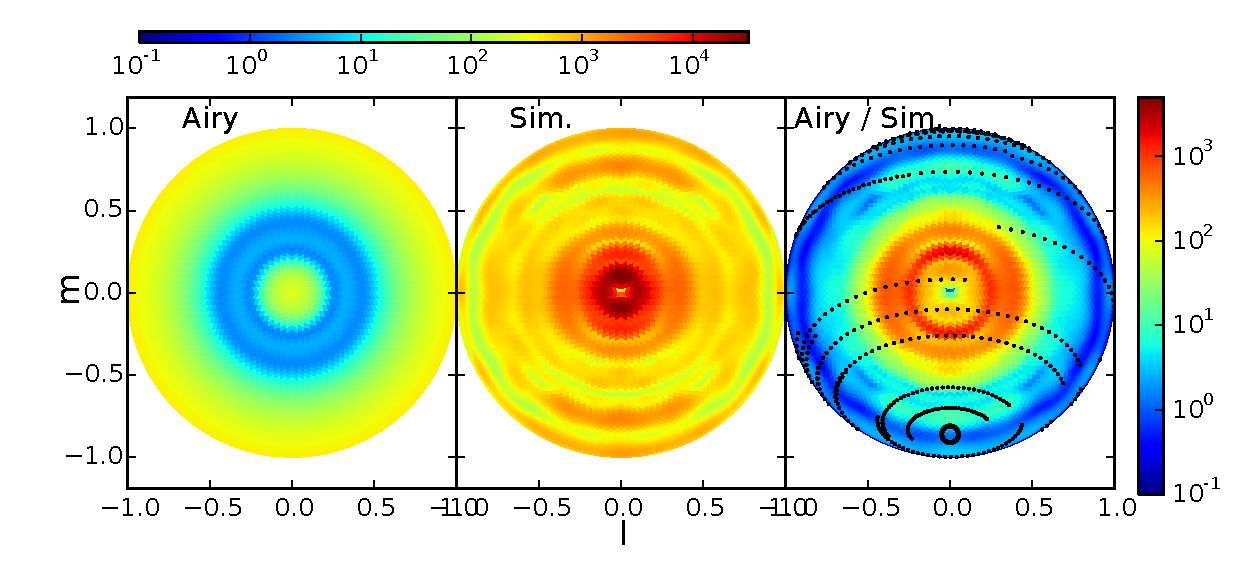
\includegraphics[width=\linewidth]{directional_high_delay_average_in_beam.eps}
\caption{All-sky directional chromaticity of antenna power pattern. }
\label{fig:directional-beam-chromaticity}
\end{figure*}

\subsection{Effect on Delay Power Spectrum}\label{sec:chromaticity-delay-spectrum}

Now we consider the effect of chromaticity of the power pattern on the delay power spectrum. 

We simulate visibilities from our foreground model using three different models for the antenna power pattern -- {\it Airy} pattern, simulated dish, and a pattern at 150~MHz of the simulated dish assumed to be achromatic over the entire band. 

Fig.~\ref{fig:asm-dps-beam-chromaticity-baselines} shows the delay power spectra of foregrounds obtained with the aforementioned models for power pattern. In all these panels, power spectra obtained with achromatic, {\it Airy} disk and simulated disk are shown in black, red, and blue respectively. The vertical gray lines denote the horizon limits for a 14.6~m antenna spacing. The full band delay power spectra of the foregrounds measured on a 14.6~m antenna spacing oriented eastward is shown in the top left panel. A clear trend of broadening of spillover-wings outside the horizon limits is seen with increasing chromaticity. For instance, the spillover from foreground delay power spectrum obtained with simulated dish pattern extends out to $k_\parallel \approx \pm 0.14\,h$~Mpc$^{-1}$, with the {\it Airy} pattern it extends out to $k_\parallel \approx \pm 0.08\,h$~Mpc$^{-1}$, while the achromatic beam extends it only out to $k_\parallel \approx \pm 0.05\,h$~Mpc$^{-1}$. Thus an increase in chromaticity extends the foreground spillover into higher $k_\parallel$-modes making them inaccessible for EoR H{\sc i} signal detection.

Following the foreground removal strategy, the top middle panel shows these foreground delay spectra deconvolved using the complex delay CLEAN algorithm \citep{tay99,par09,par12b}. The CLEAN window covers delay bins between the horizon delay limits and extends further by three delays bins on each side of the horizon limit where a delay bin is of size inverse of the bandwidth. The panel at the top right shows the residuals left behind after deconvolution. 

% \begin{figure*}[htb]
% \centering
% 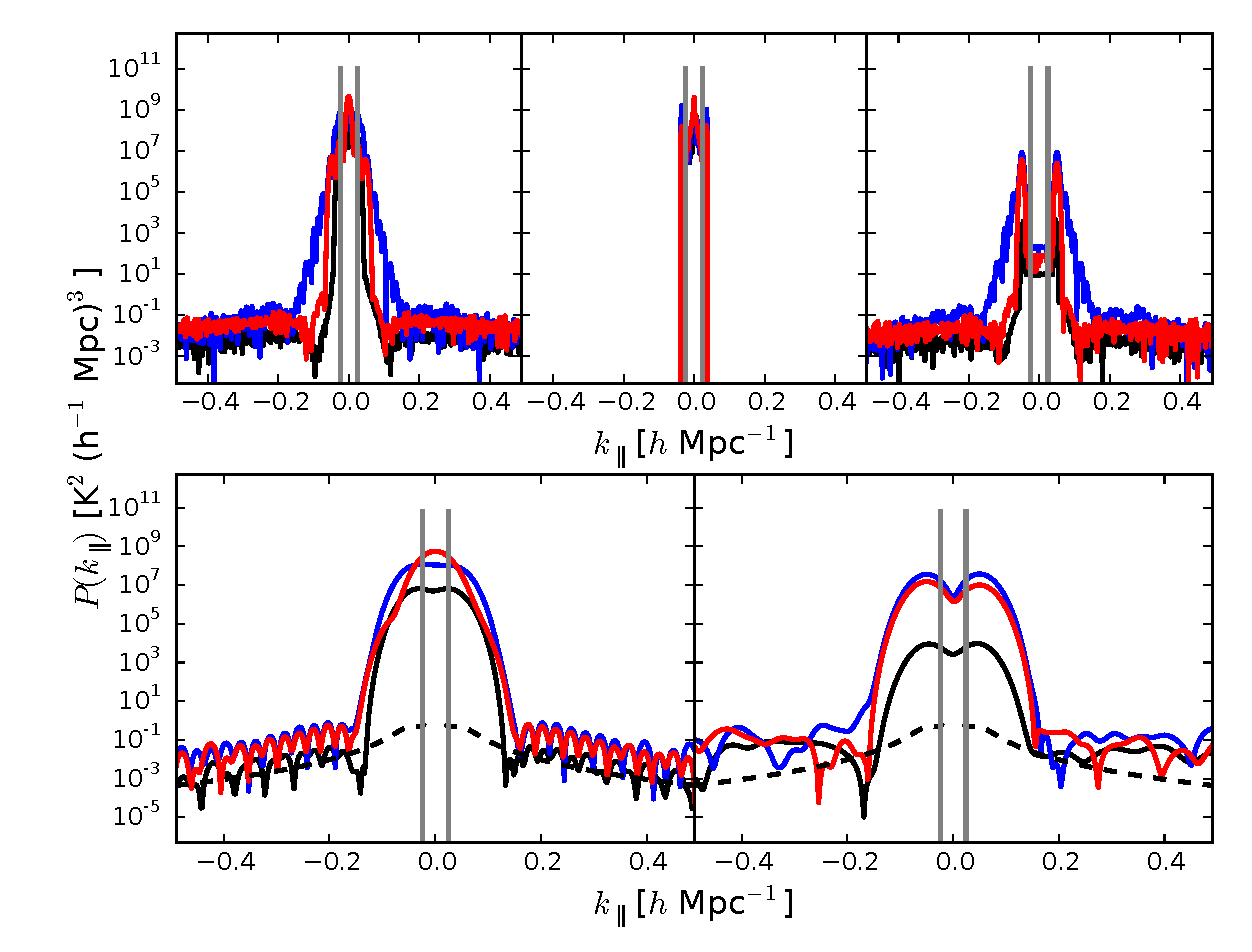
\includegraphics[width=\linewidth]{asm_beam_chromaticity_bl2_LST_3.96_hrs_subband_150.0_MHz.eps}
% \caption{Effect of chromaticity of antenna power pattern on foreground delay power spectra for a 14.6~m baseline.}
% \label{fig:asm-dps-beam-chromaticity-14.6m-baseline}
% \end{figure*}

% \begin{figure*}[htb]
% \centering
% 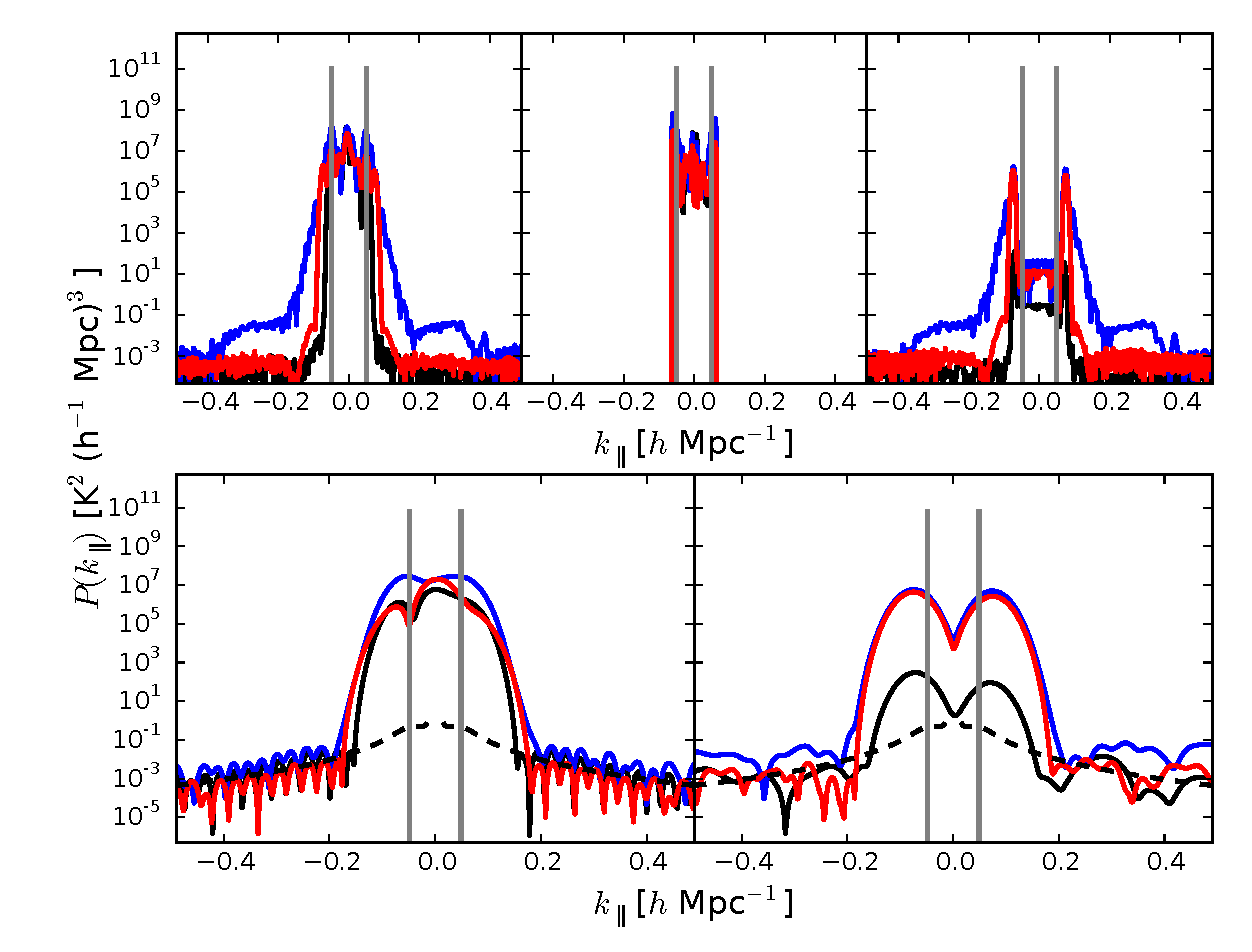
\includegraphics[width=\linewidth]{asm_beam_chromaticity_bl8_LST_3.96_hrs_subband_150.0_MHz.eps}
% \caption{Effect of chromaticity of antenna power pattern on foreground delay power spectra for a 29.2~m baseline.}
% \label{fig:asm-dps-beam-chromaticity-29.2m-baseline}
% \end{figure*}

\begin{figure*}[htb]
\centering
\includegraphics[width=\linewidth]{asm_foreground_eor_beam_chromaticity_fullband.eps}
\caption{Effect of chromaticity of antenna power pattern on foreground delay power spectra for different baselines.}
\label{fig:asm-dps-beam-chromaticity-baselines}
\end{figure*}

\begin{figure*}[htb]
\centering
\includegraphics[width=\linewidth]{sim_asm_foreground_eor_beam_chromaticity_150.0_MHz_subband.eps}
\caption{Effect of chromaticity of antenna power pattern on foreground delay power spectra obtained from the 150~MHz subband for different baseline lengths.}
\label{fig:asm-dps-beam-chromaticity-baselines-150-subband}
\end{figure*}

\begin{figure*}[htb]
\centering
\includegraphics[width=\linewidth]{sim_asm_foreground_eor_beam_chromaticity_170.0_MHz_subband.eps}
\caption{Effect of chromaticity of antenna power pattern on foreground delay power spectra obtained from the 170~MHz subband for different baseline lengths.}
\label{fig:asm-dps-beam-chromaticity-baselines-170-subband}
\end{figure*}

Owing to the chromaticity of power patterns, the spillover from foregrounds extends beyond the horizon limits, most severely in the simulated disk pattern. As a result the residuals have significant power remaining on either side of the horizon limits since the window for deconvolution is narrower than the extent of spillover along $k_\parallel$. The two peaks on either side is most severe for the simulated disk pattern followed by that for the {\it Airy} disk pattern and least for an achromatic power pattern. 

We investigate the effect of chromaticity of power pattern in a foreground avoidance strategy that avoids the aforementioned deconvolution of delay spectrum. Application of window functions with high sidelobe suppression have been discussed for mitigating foreground contamination \citep{thy13}. In line with the foreground avoidance strategy, the visibilities from the full band foreground simulation (whose delay power spectrum is shown on the top left) are multiplied by a Blackman-Harris window function of 10~MHz effective bandwidth. The delay power spectra so produced are shown in the panel on the bottom left. Due to the decreased effective bandwidth the resolution of the delay power spectrum appears decreased. Hence, only the $|k_\parallel| \gtrsim 0.14\,h$~Mpc$^{-1}$ modes remain accessible. Due to the overall lower amplitude of the {\it Airy} power pattern relative to the simulated dish power pattern and the achromatic pattern, the sidelobe levels of foreground delay power spectra from an {\it Airy} pattern are lower than the other models by almost two orders of magnitude. 

Following a delay-deconvolution based foreground removal strategy, we apply the Blackman-Harris window of effective bandwidth 10~MHz on the unsubtracted foreground residuals (top right panel) in frequency domain and obtain the delay power spectrum shown in the bottom right panel. It is noted that lesser the chromaticity the more effective the deconvolution process is in lowering the residuals in and around the horizon limits. For instance, the peak of the delay power spectrum using the achromatic beam is lowered by four orders of magnitude relative to the original peak whereas the residuals of delay power spectra with chromatic {\it Airy} and simulated power patterns is lowered only by two orders of magnitude. However, owing to the ineffective subtraction of the response extended beyond the horizon limits, the sidelobe levels have not been lowered significantly and are within an order of magnitude of each other.

In both strategies, the EoR H{\sc i} signal power spectrum obtained by simulations with 21cmFAST (Mesinger et al. 2008) is shown for reference (dashed black lines) in the bottom panels. 

\subsection{Constraints on Reflections between Antennas}\label{sec:reflectometry}

Patra~et~al.~2015 (submitted) and Ewall-Wice~et~al.~2015 (submitted) discuss the measured and simulated reflections between a dish and its feed. We provide a related discussion by estimating the attenuation in power required to keep the foreground power reflected between adjacent antennas below the expected EoR H{\sc i} signal level for the different models of power patterns used in our study.

The effect of reflections it to shift the measured foreground power to higher modes in $\tau$ (or equivalently in $k_\parallel$) and thus cause further contamination in these higher $k_\parallel$ modes which are considered sensitive for EoR H{\sc i} signal detection. Here we estimate the attenuation required at specific $k_\parallel$ modes of interest to contain reflected foreground power between antennas below expected EoR H{\sc i} power, both corresponding to a 14.6~m antenna spacing. 

We define the required attenuation as the ratio: 
\begin{align}
  \Gamma_{k_\parallel}(\tau) &= \frac{P_\textrm{H{\sc i}}(k_\parallel)}{P_\textrm{FG}(k_\parallel - \frac{\dif k_\parallel}{\dif \tau}\,\tau)},
\end{align}
where, $P_\textrm{H{\sc i}}(k_\parallel)$ is the EoR H{\sc i} power spectrum for the chosen antenna spacing, $P_\textrm{FG}(k_\parallel)$ is the foreground delay power spectrum obtained with a Blackman-Harris window function applied over the full band of the three uniquely oriented 14.6~m antenna spacings further averaged over a 0--12 hr LST range and over both positive and negative $k_\parallel$ modes, $\tau$ is the delay caused by reflections, and $\dif k_\parallel/\dif \tau$ is the {\it jacobian} in the transformation of $\tau$ to $k_\parallel$. 

Fig.~\ref{fig:fg-reflections} shows $\Gamma_{k_\parallel}(\tau)$ (in dB) for selected $k_\parallel$ at 0.08~$h$~Mpc$^{-1}$ (left), 0.1~$h$~Mpc$^{-1}$ (middle), and 0.12~$h$~Mpc$^{-1}$ (right) as a function of delays due to reflections from other antenna spacings. The light, medium and dark shaded curves show $\Gamma_{k_\parallel}(\tau)$ for achromatic, {\it Airy}, and chromatic antenna power patterns respectively. These curves set an upper limit to the reflected foreground power below the EoR H{\sc i} signal power as a function of delays caused by antenna-to-antenna reflections. It is noted that a chromatic simulated power pattern sets the most severe upper limit in all three chosen $k_\parallel$ for delays $\tau < 80$~ns (left), $\tau < 120$~ns (middle), and $\tau < 160$~ns. 

\begin{figure*}[htb]
\centering
\includegraphics[width=\linewidth]{spec_on_foreground_reflected_power_21cmfast_14.6m_150.0_MHz_subband_v2.eps}
\caption{Attenuation of foreground power (in dB) from antenna-to-antenna reflections required to keep the reflected foreground power below EoR H{\sc i} signal power.}
\label{fig:fg-reflections}
\end{figure*}

The required attenuation is also a sensitive function of the chosen $k_\parallel$ mode. For instance, at $k_\parallel=0.08\,h$~Mpc$^{-1}$, the reflections with delays 70~ns require to be attenuated by at $\gtrsim 85$~dB for the simulated power pattern, $\gtrsim 82$~dB for the {\it Airy} pattern, and $\gtrsim 70$~dB for the achromatic pattern. However, at $k_\parallel=0.1\,h$~Mpc$^{-1}$ for the same delay of reflection, the requirement on attenuation is lowered to $\gtrsim 75$~dB, $\gtrsim 30$~dB and $\gtrsim 22$~dB respectively. If the chosen $k_\parallel$ is instead 0.12~$h$~Mpc$^{-1}$, the required attenuation is further relaxed to $\gtrsim 60$~dB, $\gtrsim 15$~dB and $\gtrsim 15$~dB respectively. This further reinforces the significance of reducing the chromaticity of the antenna power pattern to further relax the constraint on the system to achieve the attenuation required to contain the reflected foreground power from other antennas from contaminating the sensitive EoR H{\sc i} signal modes in the {\it EoR window}.

\section{Summary}\label{sec:summary}

\acknowledgments

This work was supported by the U. S. National Science Foundation (NSF) through award AST-1109257. DCJ is supported by an NSF Astronomy and Astrophysics Postdoctoral Fellowship under award AST-1401708. JCP is supported by an NSF Astronomy and Astrophysics Fellowship under award AST-1302774. 

% \appendix

% \par\bigskip
\bibliographystyle{apj}
\bibliography{eor}

\end{document}
